\documentclass[10pt]{dokument-ppi}

\begin{document}


\Cwiczenie{Ćwiczenie 3}
\Meta
\Tytul{Macierz odpowiedzialności}
\Data{2012-11-21}
\Wersja{2.0}
\Autorzy{TC}
\MakeDokumentMeta


\section{Macierz odpowiedzialności}

Znajduje się na stronie \pageref{fig:macierz}.
\begin{figure}[h!]
    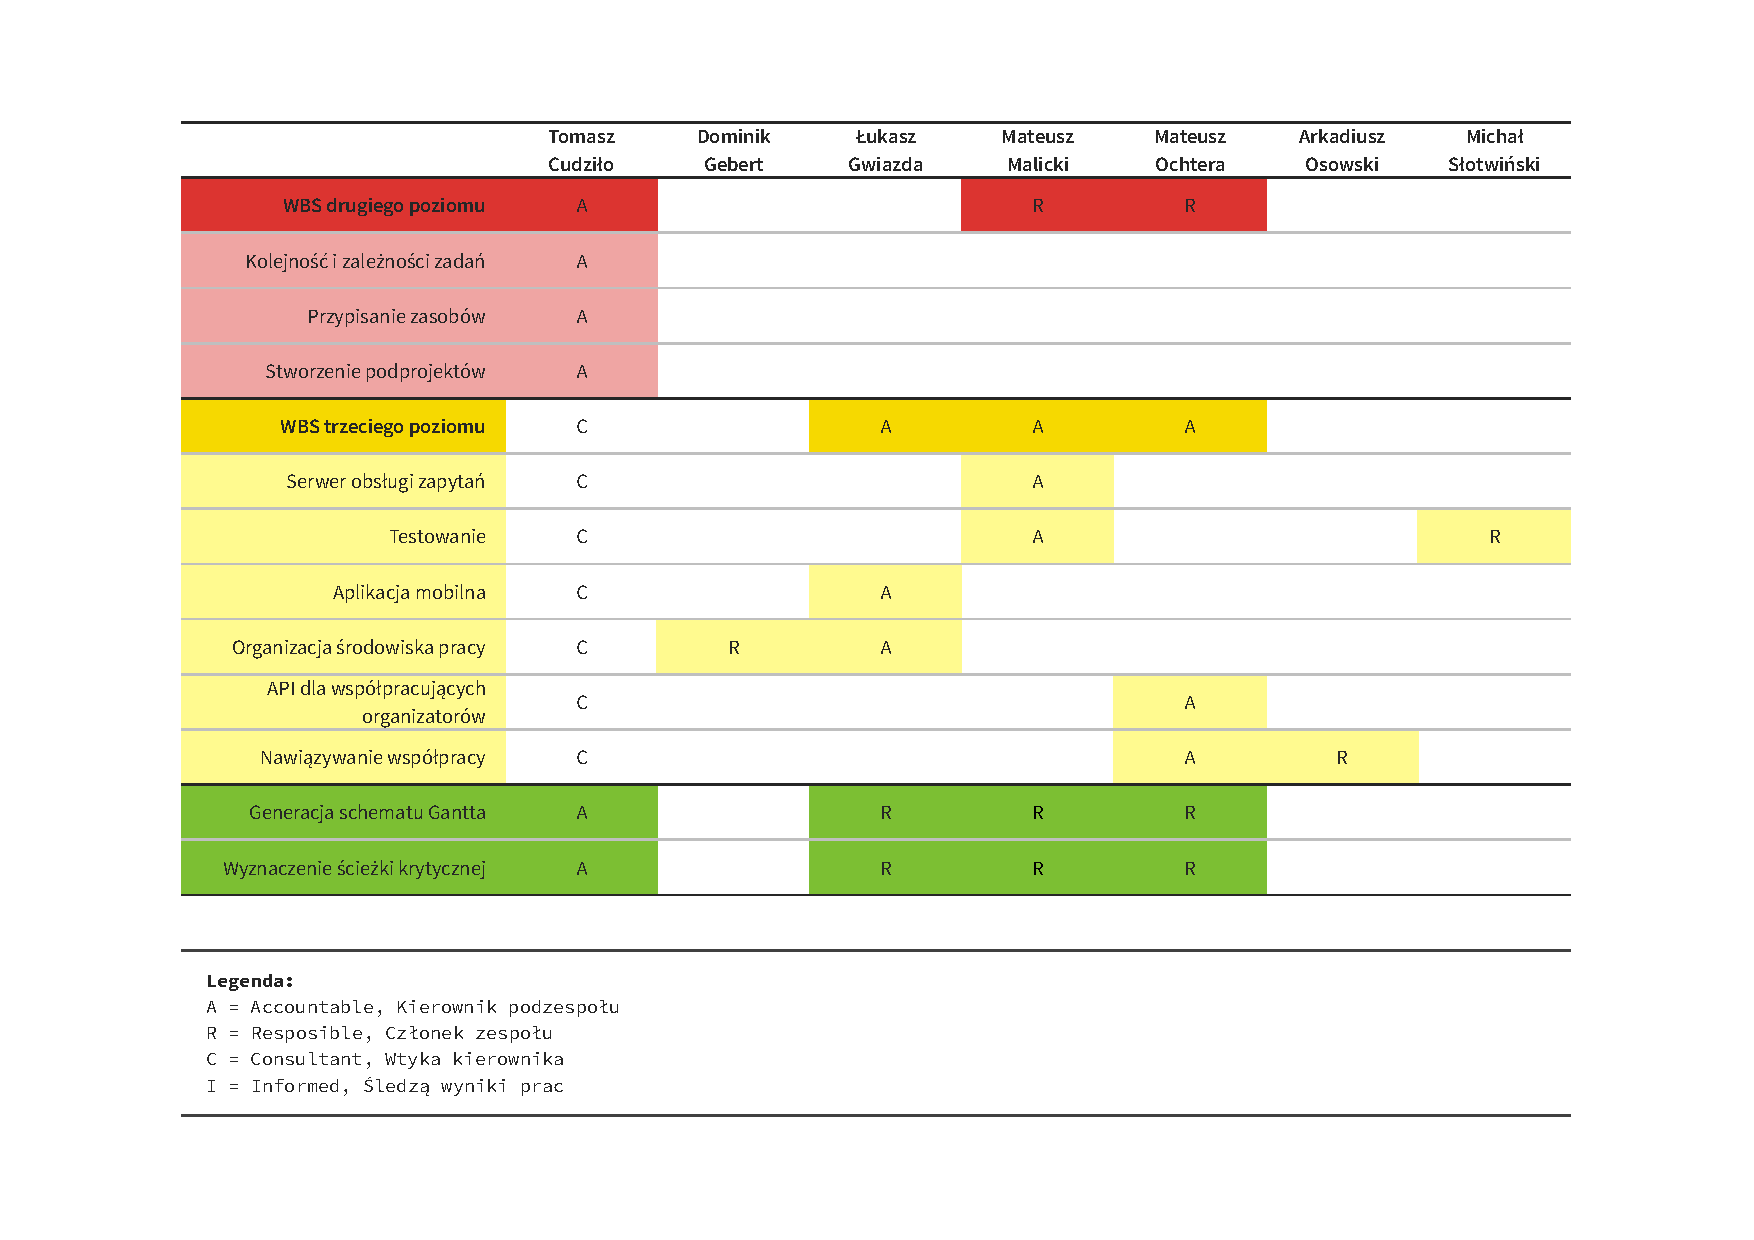
\includegraphics[trim=3cm 2cm 3cm 2cm,angle=270,width=\textwidth]{./figury/macierz-odpowiedzialnosci}
    \caption{Macierz odpowiedzialności za dokumenty tworzone w ramach ćwiczenia 3.}
    \label{fig:macierz}
\end{figure}


\section{Historia dokumentu}
\begin{versions}
    \version*{1.0}{2012-11-21}{TC}%
        Dodano pełną macierz odpowiedzialności.
    \version{1.1}{2012-11-21}{TC}%
        Poprawiono skład tekstu i macierzy.
    \version{2.0}{2012-11-24}{TC}%
        Dodano nowe podzadania \emph{Koordynacja pracy} i \emph{Administracja infrastruktury}.
\end{versions}


\end{document}
